\section{Untersuchung des Inversen Faraday-Effekts in einem Mott-Hubbard-Isolator}
\label{sec:untersuchungife}

In diesem Abschnitt wird der durch das 8N4E-System modellierte Mott-Hubbard-Isolator mit zirkular polarisiertem Licht bestrahlt,
um zu untersuchen, ob und mit welchen Abhängigkeiten der IFE in diesem Isolator auftreten kann.
Das zirkular polarisierte Licht wird dabei durch ein hochfrequent rotierendes E-Feld
\begin{align}
  \vec{E}(t) =
  \begin{pmatrix}
    A_0 \cos{\omega t} \\
    A_0 \sin{\omega t}
  \end{pmatrix}
  \label{eqn:rotefeld}
\end{align}
mit der Frequenz $\omega$ und der Amplitude $A_0$ realisiert.
In Abbildung \ref{fig:ifemott} ist eine Skizze des Systems abgebildet.
\begin{figure}
  \centering
  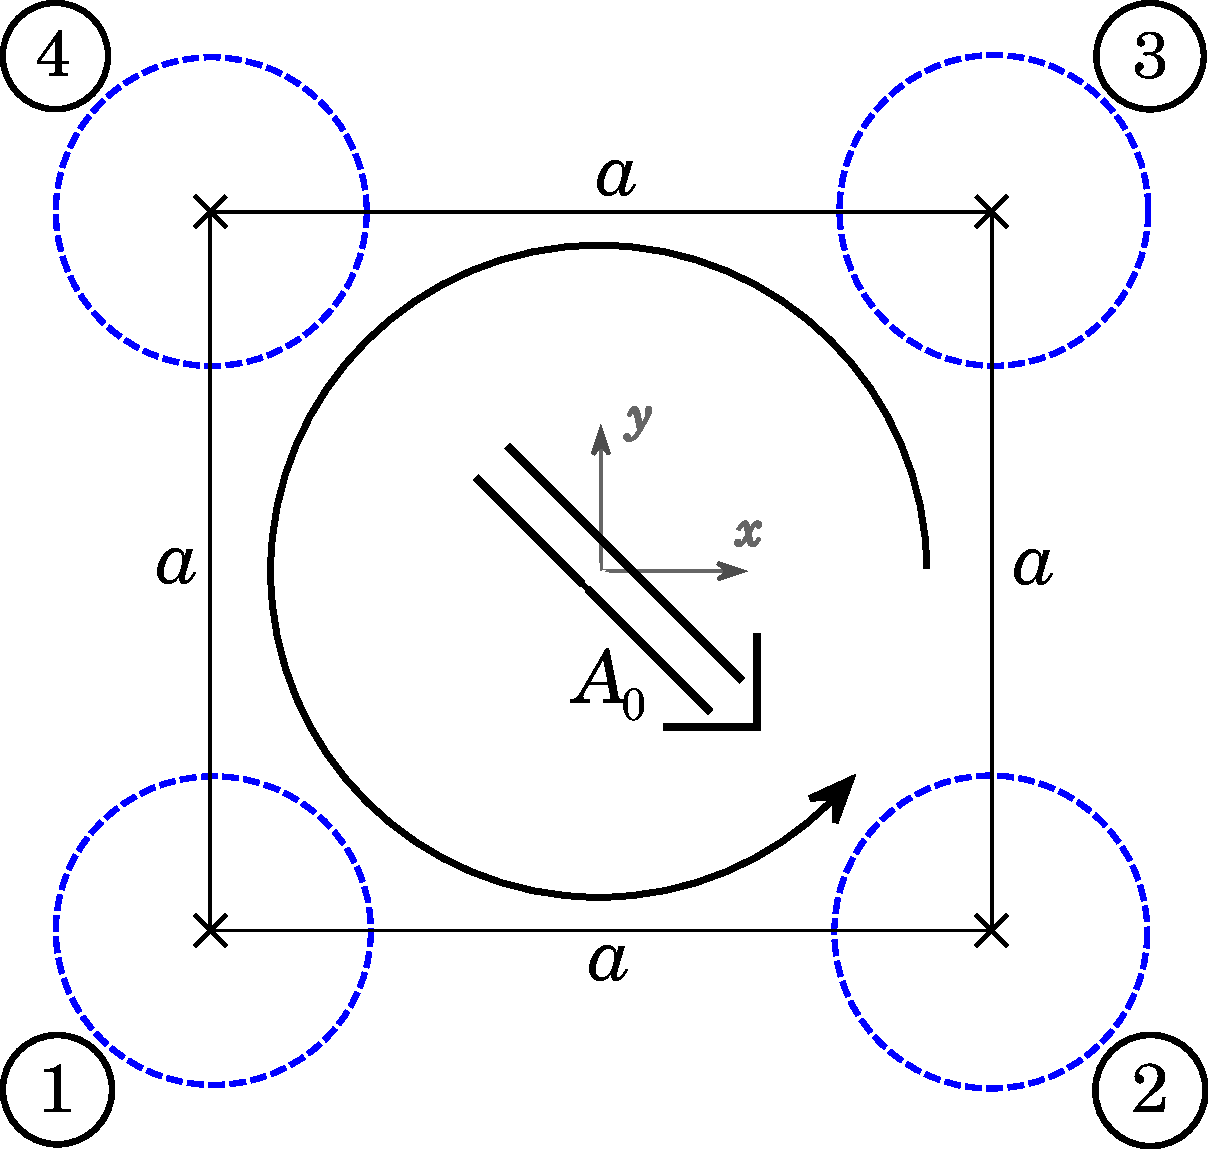
\includegraphics[height = 6cm]{Graphiken/ife_mott_system.pdf}
  \caption{Skizze des rotierenden E-Felds mit der Amplitude $A_0$ zur Modellierung des zirkular polarisierten Lichts im Mott-Hubbard-Isolator. Die Niveaus sind analog zu denen
  in Abbildung \ref{fig:hubbsystem}. Der Koordinaten-Ursprung liegt in der Mitte des Gittersystems und $a$ ist die Gitterkonstante.}
  \label{fig:ifemott}
\end{figure}
Aus dem E-Feld \eqref{eqn:rotefeld} ergibt sich durch Integration der Feldoperator in zweiter Quantisierung
\begin{align}
  H_{\Phi}(t) = q \Phi(t) & = a \sum_{i,\sigma} \left(\vec{r}_i \vec{E}(t) n_{i,\sigma}\right),
  \label{eqn:qPhi}
\end{align}
wobei $q$ die Ladung eines Elektrons, $a$ die Gitterkonstante des Systems und $\vec{r}_i$ der i-te Gitterplatz-Vektor in Einheiten von $a$ ist.
Die Gitterplatz-Vektoren sind in Gleichung \eqref{eqn:gitterplatzvektor} dargestellt. Mit den Gleichungen \eqref{eqn:hamiltonhubb} und \eqref{eqn:qPhi}
ergibt sich der zeitabhängige Hamiltonoperator für den mit zirkular polarisiertem Licht bestrahlten Mott-Isolator
\begin{align}
  H_\text{IFE}(t) = H_\text{Hubb} + a A_0 \sum_{i,\sigma} \left(\left[r_{i,x} \cos{\omega t} + r_{i,y} \sin{\omega t} \right] n_{i,\sigma}\right).
\end{align}
Die $36 \times 36$ - Hamilton-Matrix ergibt sich durch Addition der Hamilton-Matrix für den Mott-Hubbard-Isolator aus Gleichung \eqref{eqn:8N4Ehubbmatrix} mit der Hamilton-Matrix
für das zirkular polarisierte Licht. Letztere beinhaltet nur Diagonalelemente und ist in Gleichung \eqref{eqn:ifematrix} dargestellt.
Im nächsten Schritt wird die Schrödingergleichung \eqref{eqn:schroedingergleichung} wegen der Zeitabhängigkeit des Hamiltonoperators numerisch mit dem Runge-Kutta-5-Integrationsverfahren
gelöst. Dafür werden die folgenden Werte für die auftretenden Parameter eingesetzt:
\begin{align*}
  \text{Tight-Binding-Stärke}&: &J & = \SI{1}{\electronvolt} \\
  \text{Hubbard-Parameter}&: &U/J & \in \{ 4, \, 8 \} \\
  \text{Gitterkonstante}&: &a & = \SI{4e-10}{\meter} \\
  \text{Frequenz\cite{jäckl}}&: &\omega /\tfrac{J}{\hbar} & \in [0.5 , \, 2] \\
  \text{E-Feld-Amplitude\cite{jäckl}\cite{philipp}}&: &A_0 /\tfrac{J}{\symup{e}a} & \in [0.01 , \, 0.1] \\
  \text{Zeitintervall für das E-Feld\cite{jäckl}}&: &t /\tfrac{\hbar}{J} & = [0, \,76]
\end{align*}
Außerdem wird die Anfangsbedingung
\begin{align}
  \ket{\Psi(0)} = \ket{\Psi_0}
  \label{eqn:anfangsbedingung}
\end{align}
gewählt, wobei $\Psi_0$ der Grundzustand des 8N4E-Systems ohne E-Feld ist. Dieser ist für die gewählten Werte von $U/J$
in Tabelle \ref{tab:Upsi0} dargestellt.

Um den zeitabhängigen Stromerwartungswert auszurechnen wird zunächst der Stromoperator aus Gleichung \eqref{eqn:stromoperator} zu
den Basis-Zuständen \ref{tab:8N4Ehubbzust} als $36 \times 36$ - Matrix dargestellt. Diese ist in Gleichung \eqref{eqn:strommatrix} angegeben.
Daraus wird mit dem zeitentwickelten Zustand $\Psi(t)$ der Erwartungswert
\begin{align}
  I(t) = \bra{\Psi(t)} \mathcal{J} \ket{\Psi(t)}
\end{align}
für die Werte
\begin{align}
  A_0 /\tfrac{J}{\symup{e}a} & \in \{0.01,\, 0.05,\, 0.1\} & \omega /\tfrac{J}{\hbar} & \in \{0.5,\, 1.0,\, 1.5, \, 2.0\},
\end{align}
inklusive der Resonanzfrequenzen \eqref{eqn:resofreq}, bestimmt.
Es ergibt sich im gesamten Zeitintervall ein Stromerwartungswert,
der in der Größenordnung $10^{-14} \frac{J\symup{e}}{\hbar}$ liegt und daher als "numerisch Null" interpretiert wird.
Durch das zirkular polarisierte Licht wird also weder zeitabhängig, noch zeitgemittelt ein Strom oder eine Magnetisierung in dem
modellierten Mott-Hubbard-Isolator angeregt.

Um diesen Widerspruch zu der Erwartung einer endlichen Magnetisierung aus Abschnitt \ref{sec:ifeiso} zu erklären, ist in Betracht zu ziehen,
dass das betrachtete Festkörpersystem nicht ausreichend komplex ist, um durch den IFE angeregt zu werden.
Zur Überprüfung dieser Aussage wird im nächsten Schritt der Stromerwartungswert des 8N4E-Systems bei Einschalten des rotierenden E-Felds für $U/J = 0$ untersucht.
In dem Fall, dass das System ausreichend groß ist, um durch den IFE angeregt zu werden, sollte bei $U/J = 0$ ein ein endlicher, stationärer Strom erwartet,
da das System in diesem Fall keinen Mott-Isolator, sondern eher ein leitendes Material modelliert.
Da die Grundzustandsenergie bei $U/J = 0$ vierfach entartet ist, existieren vier unterschiedliche Grundzustände, für die jeweils getrennt
der Stromerwartungswert berechnet wird. Aus dem arithmetischen Mittel der berechneten Erwartungswerte ergibt sich der gesamte
Stromerwartungswert $I(t)$ in Einheiten von $\frac{J\symup{e}}{\hbar}$. Dieser ist in Abbildung \ref{fig:U0plot} gegen die Zeit $t/\tfrac{\hbar}{J}$ aufgetragen.

\begin{figure}
  \centering
  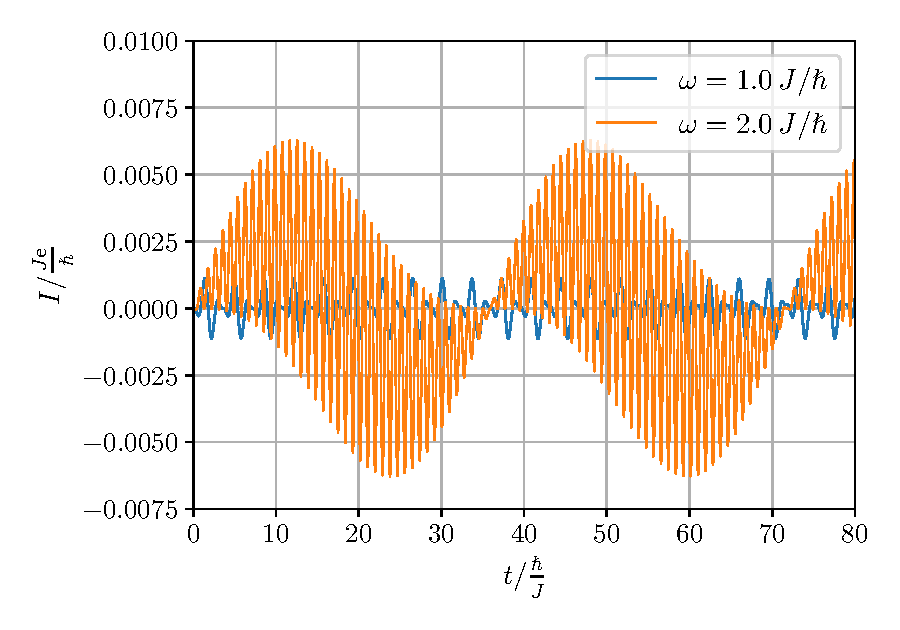
\includegraphics[height=8.0cm]{Plots/U0_E01_schoen.pdf}
  \caption{Stromerwartungswert in Abhängigkeit von der Zeit für zwei verschiedene Frequenzen, wobei $U/J = 0$ und $A_0 = 0.05 \tfrac{J}{\symup{e}a}$ ist.
  Bei $\omega = 2.0\tfrac{J}{\hbar}$ liegt eine Resonanzfrequenz des Systems.}
  \label{fig:U0plot}
\end{figure}

Für die Entstehung der Magnetisierung ist ausschließlich der stationäre, nicht oszillierende Teil des Stroms, der sich aus einer Zeitmittelung ergibt, relevant.
Aus Abbildung \ref{fig:U0plot} ist entnehmbar, dass der Stromerwartungswert periodisch um Null oszilliert und im Langzeitmittel verschwindet. Dies wird für
das Zeitintervall $T/\tfrac{\hbar}{J} \in [0,300]$ numerisch bestätigt.
Es wird daher kein stationärer Kreisstrom durch das zirkular polarisierte Licht mittels des IFE induziert, obwohl das Festkörpersystem bei $U/J = 0$ keinen Mott-Isolator
repräsentiert. Dadurch wird die Behauptung, dass der modellierte Festkörper, bestehend aus vier Gitterplätzen, zu klein für die Untersuchung des IFE ist, gestützt.

Ein weiterer Aspekt, welcher für die Beobachtung eine Rolle spielen könnte, ist die Teilchen-Loch-Symmetrie im System.
Diese wird in der folgenden Betrachtung gebrochen, indem eine Übernächst-Nachbar-Tight-Binding-Wechselwirkung im modellierten Mott-Hubbard-Isolator
ergänzt wird. Dazu werden zusätzliche Tight-Binding-Terme, die das Springen der Elektronen zwischen den Gitterplätzen 1 und 3 bzw. 2 und 4
mit der Stärke $\lambda = 0.2 J$ ermöglichen, ergänzt. Daraus und aus Gleichung \eqref{eqn:hamiltonhubb} ergibt sich der um die Übernächst-Nachbar-Tight-Binding-Wechselwirkung erweiterte Hamiltonoperator
\begin{align}
  H_\text{TL} = H_\text{Hubb} + H_\text{Diag} = H_\text{Hubb} - \lambda \sum_{i=1}^2 \sum_{\sigma} \left(c_{i+2,\sigma}^{\dag}c_{i,\sigma}^{\phantom{\dag}} + c_{i,\sigma}^{\dag}c_{i+2,\sigma}^{\phantom{\dag}} \right).
\end{align}
Mit Hilfe der Basis-Zustände aus Tabelle \ref{tab:8N4Ehubbzust} wird dieser in die Matrix-Darstellung gebracht. Die berechneten $36 \times 36$ - Matrizen für $H_\text{Diag}$ und $H_\text{Hubb}$ sind in den Gleichungen
\eqref{eqn:elmatrix} und \eqref{eqn:8N4Ehubbmatrix} angegeben.
Analog zum ersten Teil dieses Abschnitts wird im System ein hochfrequent rotierendes E-Feld hinzugefügt und der Stromerwartungswert für diverse Parameter berechnet. Im gesamten Zeitintervall ergibt sich
ein Strom, der in der Größenordnung $10^{-15} \frac{J\symup{e}}{\hbar}$ liegt, und daher als "numerisch Null" interpretiert wird. Die im modellierten Mott-Hubbard-Isolator vorhandene
Teilchen-Loch-Symmetrie wird daher nicht für die Beobachtung, dass kein Strom mittels des IFE im System angeregt wird, verantwortlich gemacht.

Die vorangegangenen Untersuchungen deuten darauf hin, dass das betrachtete Festkörpersystem zu klein für die Untersuchung des IFE ist.
Dennoch ist nicht auszuschließen, dass durch die erzielten Ergebnisse die Realität abgebildet wird, sodass in einem Mott-Isolator kein
Kreisstrom durch den IFE angeregt werden kann.
In der in Abschnitt \ref{sec:ifeiso} vorgestellten Herleitung des IFE in Isolatoren werden einige anzweifelbare Annahmen getroffen.
Vor allem die Vernachlässigung von quantenmechanischen Effekten kann in Frage gestellt werden,
da beispielsweise das Vorhandensein des Pauli-Prinzips die Dynamik der Elektronen erheblich beeinflusst kann.
Somit ist nicht eindeutig klar, wie der Widerspruch zwischen der analytischen Herleitung aus Abschnitt \ref{sec:ifeiso} und den Ergebnissen zustande kommt.
